\documentclass{beamer}

\usepackage{lmodern}
\usepackage{booktabs}
\usepackage{listings}
\beamertemplatenavigationsymbolsempty

\title{~\\ ~\\ ~\\ Trusted DCR: Decentralised workflow management in a byzantine setting}
\author{Mikkel Gaub \and Malthe Ettrup Kirkbro \and Mads Frederik Madsen}
\date{~\\ ~\\ ~\\ \center June 21, 2018 }

\usetheme{metropolis}

\def \emptysubtitle {}
\addtobeamertemplate{frametitle}{}{%
  \ifx\insertframesubtitle \emptysubtitle%
	\vspace*{-6ex}
  \begin{beamercolorbox}[wd=\paperwidth,ht=5ex,dp=3ex,left]{frametitle}%
	 	\hspace*{2ex}\insertframetitle%
	\end{beamercolorbox}%
  \else%
	\vspace*{-1ex}
  \usebeamerfont{framesubtitle}%
  \begin{beamercolorbox}[wd=\paperwidth,ht=2ex,dp=2ex,left]{framesubtitle}%
	 	\hspace*{2.67ex}\insertframesubtitle%
	\end{beamercolorbox}%
  \fi%
}

\begin{document}
\maketitle

\begin{frame}{Introduction}%frederik
%contributions
%
    \begin{itemize}
    	\item
    \end{itemize}
\end{frame}

\begin{frame}{Overview}%frederik
	\begin{itemize}
\item Problem
\item Intel Software Guard Extensions
\item Transforming byzantine faults
\item Dynamic Condition Response graphs
\item Execution ordering
\item Global history
\item Cluster consensus
\item Trusted DCR
\item Implementation
\item Demo
\item Performance
\item Security
\item Smart contracts
	\end{itemize}
\end{frame}

\begin{frame}{Problem}%frederik
\begin{itemize}
	\item Create a fault tolerant decentralised DCR engine:

	\vfill

	\begin{itemize}
		\item High degree of concurrency

		\vfill

		\item Scalable (less than $O(n)$ messages per execution)

		\vfill

		\item Byzantine fault tolerant
	\end{itemize}
\end{itemize}
	% skriv problem
	% kontekstualisér
\end{frame}

\begin{frame}{Intel Software Guard Extensions}{SGX}%frederik
	\begin{itemize}
		\item Hardware-based Trusted Execution Environment
		\begin{itemize}
			\item Protected CPU-instructions
			\item Protected cryptographic keys in fuse arrays
		\end{itemize}

		\vfill

		\item Enclaves:
		\begin{itemize}
			\item Isolated memory and process
			\item Guaranteed integrity and confidentiality of enclave (by Intel)
		\end{itemize}

		\vfill

		\item Attestation:
			\begin{itemize}
				\item Local: Allows enclave process to verify if other local processes are running in identical enclave
				\item Remote: Allows enclave process to verify if other remote processes are running in identical enclave
			\end{itemize}
	\end{itemize}
	% Integrity protection
	% Confidentiality protection
  % Remote attestation
\end{frame}

\begin{frame}{Intel Software Guard Extensions}{Integrity}
    \begin{itemize}
    	\item Integrity is guaranteed by:

			\vfill

    	\begin{itemize}
    		\item Enclave mode (process bit) %SECS?

  			\vfill

    		\item Processor Reserved Memory (PRM)

  			\vfill

    		\item Enclave Page Cache (EPC)

  			\vfill

    		\item Cryptographically signed when on persistent storage

  			\vfill

    		\item Merkle-Tree of MACs of memory, with root in processor internal memory
    	\end{itemize}
    \end{itemize}
\end{frame}

\begin{frame}{Intel Software Guard Extensions}{Confidentiality}
    \begin{itemize}
    	\item Confidentiality is guaranteed by:

			\vfill

    	\begin{itemize}
    		\item Enclave mode (process bit)

  			\vfill

    		\item Processor Reserved Memory (PRM)

  			\vfill

    		\item Enclave Page Cache (EPC)

  			\vfill

    		\item Encrypted memory
    	\end{itemize}
    \end{itemize}
\end{frame}

% \begin{frame}{Intel Software Guard Extensions}{Local attestation}

% \end{frame}

\begin{frame}{Intel Software Guard Extensions}{Remote attestation}
	\begin{itemize}

		\vfill

		\item Requires an EPID private key
		% \begin{itemize}
		% 	\item One public key, many private keys
		% 	\item Intel provisions this key during first SGX run
		% \end{itemize}

		\vfill

		\item Quoting Enclave (QE) locally attests enclave

		\vfill

		\item On local attestation, QE signs the attestation with EPID private key

		\vfill

		\item When received by a remote enclave:
    \begin{itemize}
       \item The attestation will uniquely identify the enclave
       \item The signature will prove that a QE has locally attested it
     \end{itemize}

		\vfill

		\item In practice, remote attestation requires contact to Intel server:%
    \begin{itemize}
       \item Revocation of leaked private keys
     \end{itemize} 
	\end{itemize}
\end{frame}

\begin{frame}{Transforming byzantine faults}{Idea} %Frederik
  \begin{itemize}
  	\item Given integrity, confidentiality and remote attestation from SGX

  	\vfill

  	\item We can make a transformation of distributed protocols

  	\vfill

  	\item Crash-fault tolerant to byzantine fault tolerant
  	\begin{itemize}
  		\item Must handle unreliable channels
  	\end{itemize}
  \end{itemize}
\end{frame}

\begin{frame}{Transforming byzantine faults}{Intuition}
	\begin{itemize}
		\item Integrity protects enclaves from experiencing byzantine faults

  	\vfill

		\item Confidentiality protects enclaves from other components

  	\vfill

		\item With a byzantine protected subprocess, other subprocesses can be protected through that

	\end{itemize}
\end{frame}

\begin{frame}{Transforming byzantine faults}{Simple overview}
	\begin{itemize}
		\item Run the core of the protocol in an SGX enclave

  	\vfill

		\item Add message passing subprocesses outside the enclave

  	\vfill

		\item Provision enclaves with symmetric key through remote attestation

  	\vfill

		\item MAC each sent message with the shared key

  	\vfill

		\item Verify MAC upon receival of message

  	\vfill

		\item Integrity guarantees that the enclave does not sign message after experiencing byzantine fault

  	\vfill

  	\item Confidentiality guarantees that other components cannot access the shared key

	\end{itemize}
\end{frame}

\begin{frame}{Transforming byzantine faults}{Result}
	\begin{itemize}
		\item On byzantine errors in the wrapper components, it can at most drop, redirect or corrupt messages
		\begin{itemize}
			\item Redirects are handled by unique ids, and will be dropped by the receiving enclave
			\item Corrupted messages will be dropped by the enclave
			\item So this is equivalent to dropped messages
		\end{itemize}

	\vfill

		\item On byzantine errors in the enclave components, the integrity guarantee will ensure wrong/no MACing of messages
		\begin{itemize}
			\item Either the enclave infinitely retries MAC attempts (crash), or wrongly MACed messages will be dropped
		\end{itemize}
	\end{itemize}
\end{frame}

\begin{frame}{Dynamic Condition Response graphs}{Basics}%frederik
	\begin{tabular}{lc}
	  \parbox{0.5\linewidth}{\begin{itemize}
			\item Declarative graph representation of a workflow	
			\vfill
			\item Events: nodes representing possible events and actions of the workflow
			\vfill
			\item Relations: directed edges representing constraints and effects in the workflow
		\end{itemize}
		}
		&
	  \parbox{0.5\linewidth}{
		\begin{figure}[p]
			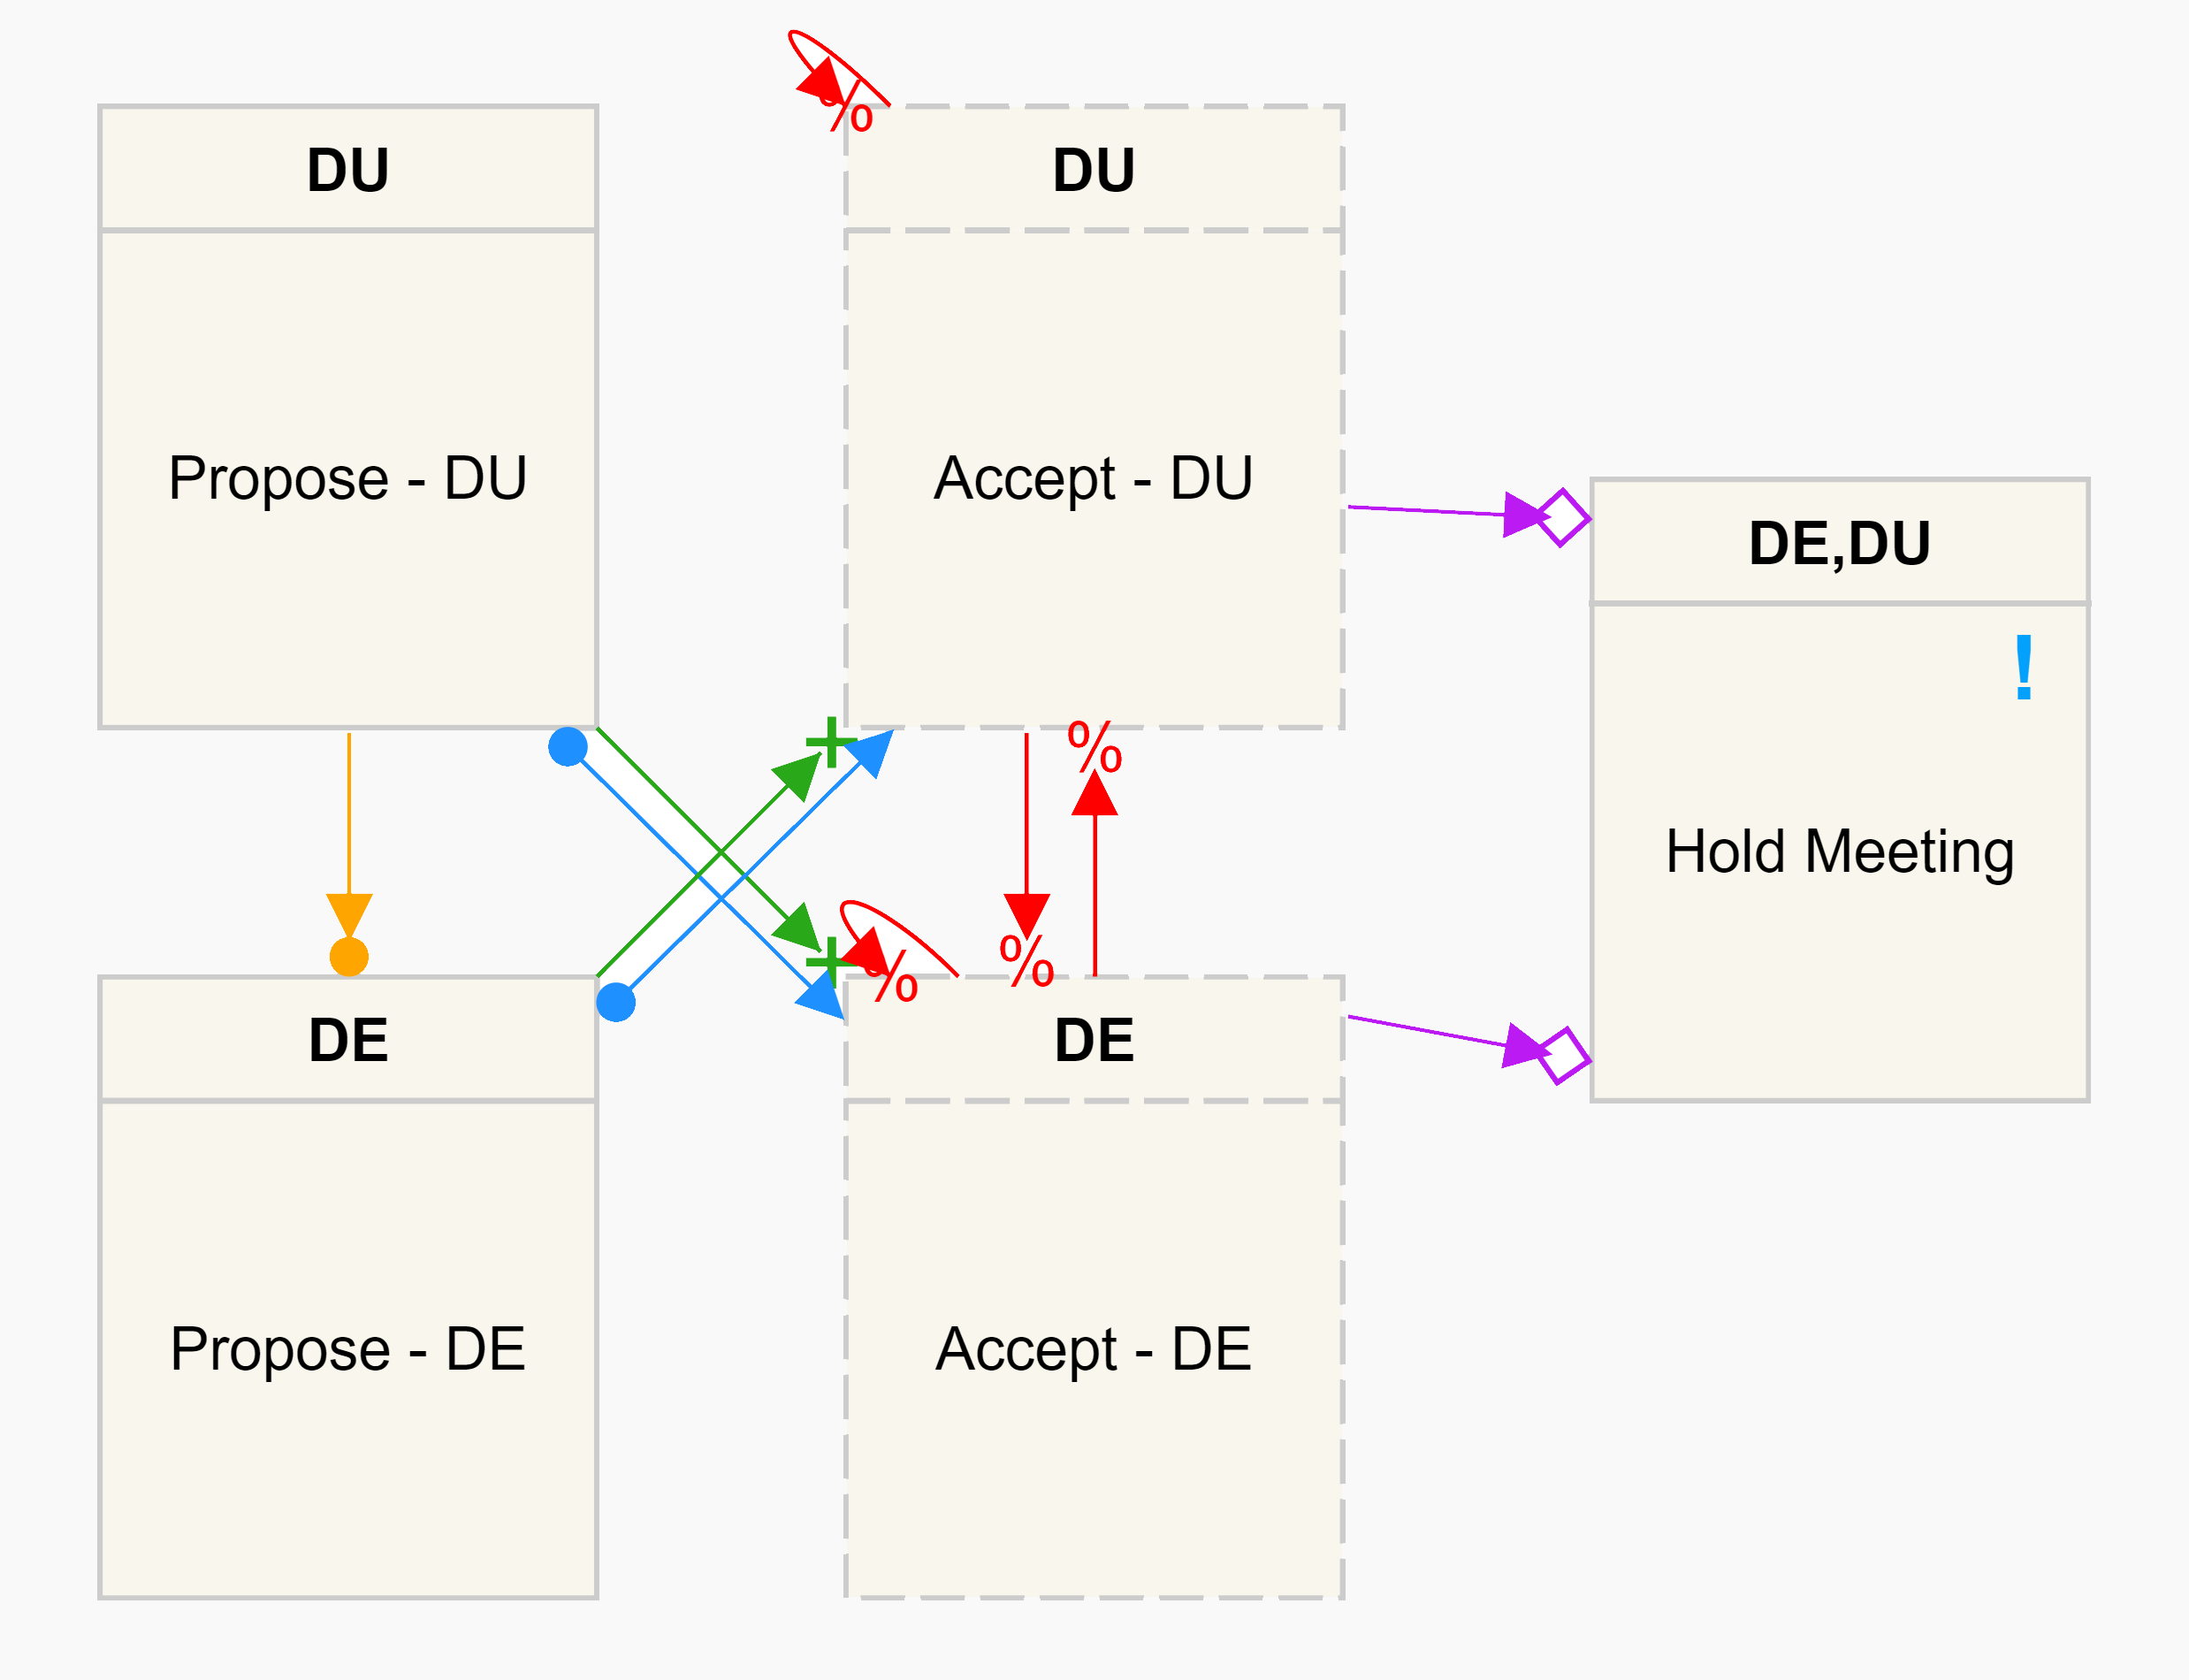
\includegraphics[scale=0.08]{figures/example6.png}
		\end{figure}
		}
	\end{tabular}
	% Workflow
	% events
	% relations (directed edges)
	% eksempel
	% concurrency
\end{frame}

\begin{frame}{Dynamic Condition Response graphs}{Concurrency}
	\begin{itemize}
		\item Dynamic independency:
		\begin{itemize}
			\item In given graph state $G$: $E(E(G, e_1),e_2)=E(E(G, e_2),e_1)$
		\end{itemize}

		\vfill

		\item Static independency:
		\begin{itemize}
			\item Dynamic independency in any \textit{reachable} state from $G$
		\end{itemize}

		\vfill

		\item Approximate static independency:
		\begin{itemize}
		 	\item Dynamic independency for \textit{any} state of $G$
		 	\item Seems harder, but is easier, because it can be calculated only using the relations, disregarding the events' state
		\end{itemize}

		\vfill

		\item Dynamic independency allows for more concurrency
  \end{itemize}
\end{frame}

\begin{frame}{Execution ordering}{Race condition}%mikkel
	\begin{itemize}
		\item Ordering is needed when executions affect the same state
	\end{itemize}
	\vspace{\fill}
	\centering
    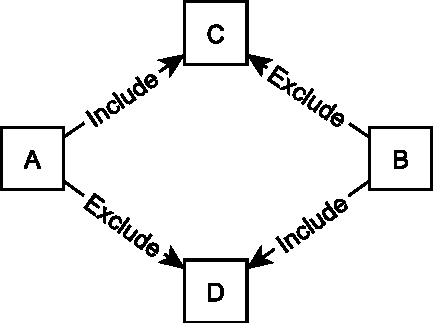
\includegraphics[scale=0.5]{figures/race-condition.pdf}
    \vspace{\fill}
    \begin{itemize}
    	\item First degree out: $N_{out}(e) \cup e$
    \end{itemize}
\end{frame}

\begin{frame}{Execution ordering}{Enabledness}%mikkel
	\begin{itemize}
		\item Ordering is needed when enabledness is affected
	\end{itemize}
	\vspace{\fill}
	\centering
    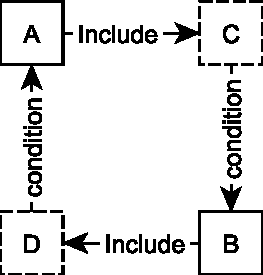
\includegraphics[scale=0.5]{figures/second-degree-effect.pdf}
    \vspace{\fill}
    \begin{itemize}
    	\item First degree: $N_{out}(e) \cup N_{in}(e) \cup e$
    	\item Second degree out: $N_{out}(N_{out}(e)) \cup N_{out}(e) \cup e$
    \end{itemize}
\end{frame}

\begin{frame}{Execution ordering}{Minimizing}%mikkel
	\begin{itemize}
		\item Second degree out has advantages with regards to optimization
	\end{itemize}
	\vspace{\fill}
	\centering
    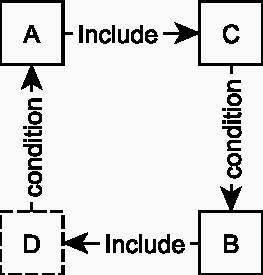
\includegraphics[scale=0.5]{figures/second-degree-no-effect.pdf}
    \vspace{\fill}
    \begin{itemize}
    	\item First degree: $N_{out}(e) \cup N_{in}(e) \cup e$
    	\item Second degree out: $N_{out}(N_{out}(e)) \cup N_{out}(e) \cup e$
    \end{itemize}
\end{frame}

\begin{frame}{Global history}{Collection}%mikkel
    \begin{itemize}
    	\item Observed executions returned from each event
    \end{itemize}
    \vspace{\fill}
    \centering
    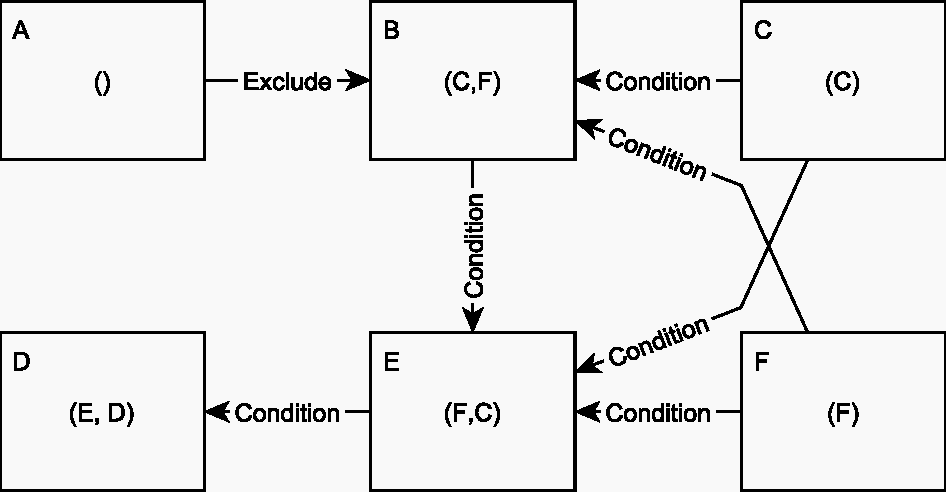
\includegraphics[scale=0.5]{figures/inconsistent-cut.pdf}
\end{frame}

\begin{frame}{Global history}{Consistent cut}
	\centering
    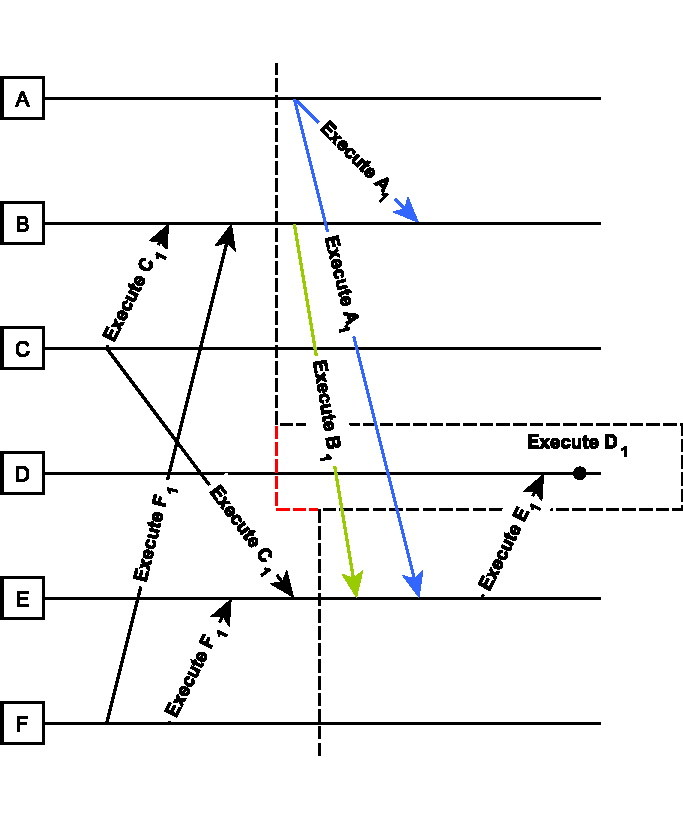
\includegraphics[scale=0.6]{figures/consistent-cut.pdf}
\end{frame}

\begin{frame}{Global history}{Ordering}
    \centering
    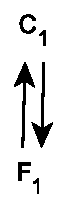
\includegraphics[scale=0.7]{figures/cut-graph.pdf}
    \vspace{\fill}
    \begin{itemize}
    	\item Topological order with arbitrary tie-breaking on cycles.
    	\item Valid runs: $(C_1, F_1)$ or $(F_1, C_1)$
    \end{itemize}
\end{frame}

\begin{frame}{Cluster consensus}%mikkel
\resizebox{\textwidth}{!}{
	\begin{tabular}{l p{3cm} p{1.5cm} l p{1.7cm}}
        \toprule
    	\textbf{Algorithm} 								& \textbf{FT: liveness} & \textbf{Recovery} & \textbf{Msgs/execution}  & \textbf{FT} \\
        \midrule
    	PBFT               	& $f = \lfloor \frac{n-1}{3} \rfloor$ & $(2f+1)^2$              & $(2f+1)+(2f+1)^2$            & Byzantine 				     \\
    	MinBFT           	& $f = \lfloor \frac{n-1}{2} \rfloor$ & $(f+1)^2$               & $2(f+1)+(f+1)^2$             & Byzantine 				     \\
    	FastBFT           	& $f = \lfloor \frac{n-1}{2} \rfloor$ & $(f+1)^2$               & $4(f+1)$                     & Byzantine 				     \\
    	Chandra-Toueg    	& $f = \lfloor \frac{n-1}{2} \rfloor$ & $0$                     & $4(f+1)+(f+1)^2$             & Crash                         \\
    	Paxos  				& $f = \lfloor \frac{n-1}{2} \rfloor$ & $0$                     & $4(f+1) + 2$                 & Crash                         \\
    	Raft               	& $f = \lfloor \frac{n-1}{2} \rfloor$ & $2(f+1)$                & $2(f+1)$                     & Crash                         \\
        \bottomrule
	\end{tabular}
	}
\end{frame}

\begin{frame}{Trusted DCR}{Raft}%malthe
  \begin{itemize}
    \item Variant of multi-Paxos
    \begin{itemize}
      \item Crash-failures
      \item $n = 2f+1$
    \end{itemize}

    \vfill

    \item Election
    \begin{itemize}
      \item Triggered by semi-random timeout
      \item Single winner or stalemate
    \end{itemize}

    \vfill

    \item Leadership
    \begin{itemize}
      \item Accept client commands
      \item Two-phase commit with quorum
    \end{itemize}
  \end{itemize}

  % Raft
  % Overlay algorithm
  % Correctness figure
\end{frame}

\begin{frame}{Trusted DCR}{Protocol}%malthe
  \begin{itemize}
    \item Entirely defined as modified Raft leader behavior
    \item Three command types: \textbf{\texttt{LOCK}}, \textbf{\texttt{EXEC}} and \textbf{\texttt{ABORT}}

    \vfill

    \item Leader algorithm
    \begin{enumerate}
      \item Client commands \textbf{\texttt{LOCK}}
      \item Leader commits \textbf{\texttt{LOCK}} in quorum
      \item Leader commands \textbf{\texttt{LOCK}} in lock-set
      \begin{itemize}
        \item Unanimous ACK: Leader commits and commands \textbf{\texttt{EXEC}} in quorum and lock-set
        \item Single NACK: Leader commits and commands \textbf{\texttt{ABORT}} in quorum and lock-set
      \end{itemize}
    \end{enumerate}
  \end{itemize}
\end{frame}

\begin{frame}{Trusted DCR}{Termination}%malthe
  \vfill
  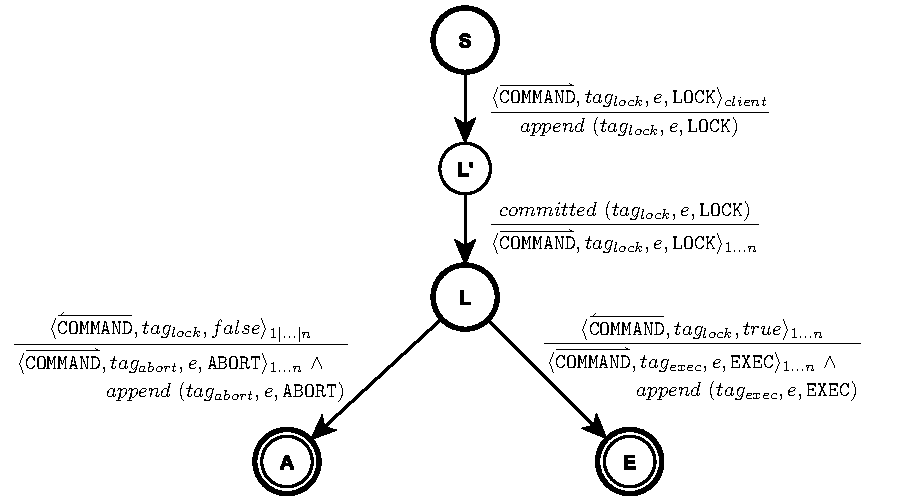
\includegraphics[width=\textwidth]{figures/raft-2pc.pdf}
  \vfill
\end{frame}

\begin{frame}{Implementation}%Malthe
  \vfill
  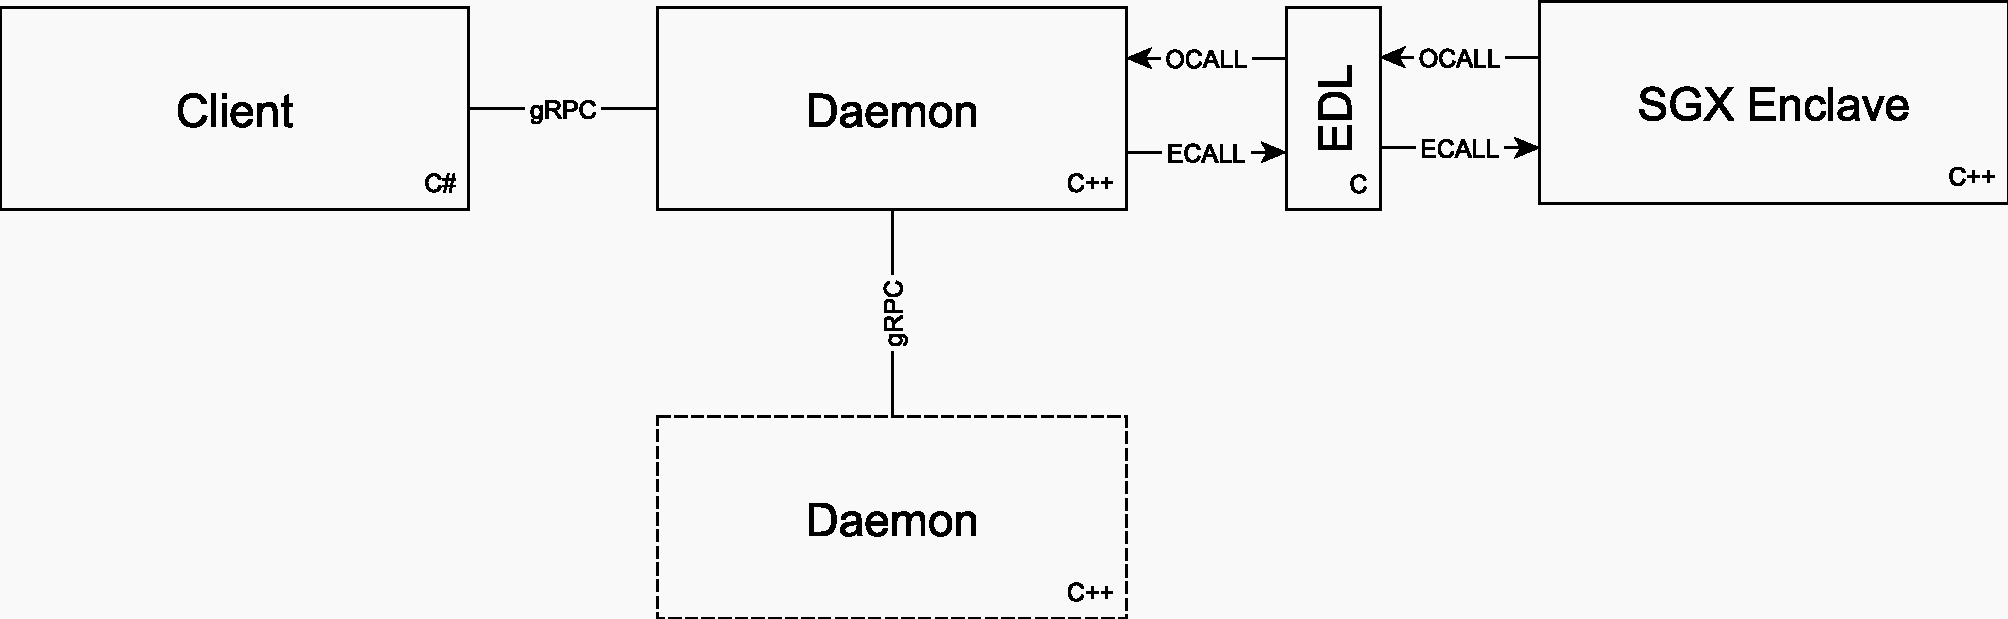
\includegraphics[width=\textwidth]{figures/network-stack.pdf}
  \vfill
\end{frame}

\begin{frame}{Demo}%Malthe

\end{frame}

\begin{frame}{Performance}%Malthe

\end{frame}

\begin{frame}{Security}{Known vulnerabilities}%Malthe
  \begin{itemize}
    \item Confidentiality
    \begin{itemize}
      \item Spectre exploit on SGX (SgxPectre)
      \item Various leaks under data-dependent memory access
    \end{itemize}

    \vfill

    \item Integrity
    \begin{itemize}
      \item Row hammer
      \item Various physical attacks
    \end{itemize}
  \end{itemize}
\end{frame}

\begin{frame}[fragile]{Security}{Pitfalls}%Malthe
  \vfill
  \begin{lstlisting}[language=C, basicstyle=\footnotesize\ttfamily, keywordstyle=\color{mLightBrown}]
struct some_struct {
  char a;
  int b;
}
...
some_struct s { 123, 999999 };
OCALL(s);
...
  \end{lstlisting}
  \vfill
\end{frame}

\begin{frame}[fragile]{Security}{Pitfalls}%Malthe
  \vfill
  \begin{lstlisting}[language=C, basicstyle=\footnotesize\ttfamily, keywordstyle=\color{mLightBrown}, commentstyle=\color{gray}]
struct append_req_t {
  ...
  entry_t* entries;
  uint32_t entries_n;
  ...
}

// ECALL
void recv_append_req(append_req_t req) {
  // req.entries points to unprotected memory here

  // copy entries to protected memory
  entry_t* prot_entries = new entry_t[req.entries_n];
  memcpy(prot_entries, req.entries,
         sizeof(entry_t) * req.entries_n);
  ...
}
  \end{lstlisting}
  \vfill
\end{frame}

\begin{frame}{Smart contracts}{Transformation}%mikkel
    \begin{itemize}
    	\item Events containing arbitrary state
    	\vfill
    	\item Effects changing arbitrary state
    	\vfill
    	\item Constraints checking arbitrary state
    	\vfill
    	\item The DAO
    \end{itemize}
\end{frame}

\begin{frame}{Smart contracts}{Simple DAO}
	\centering
	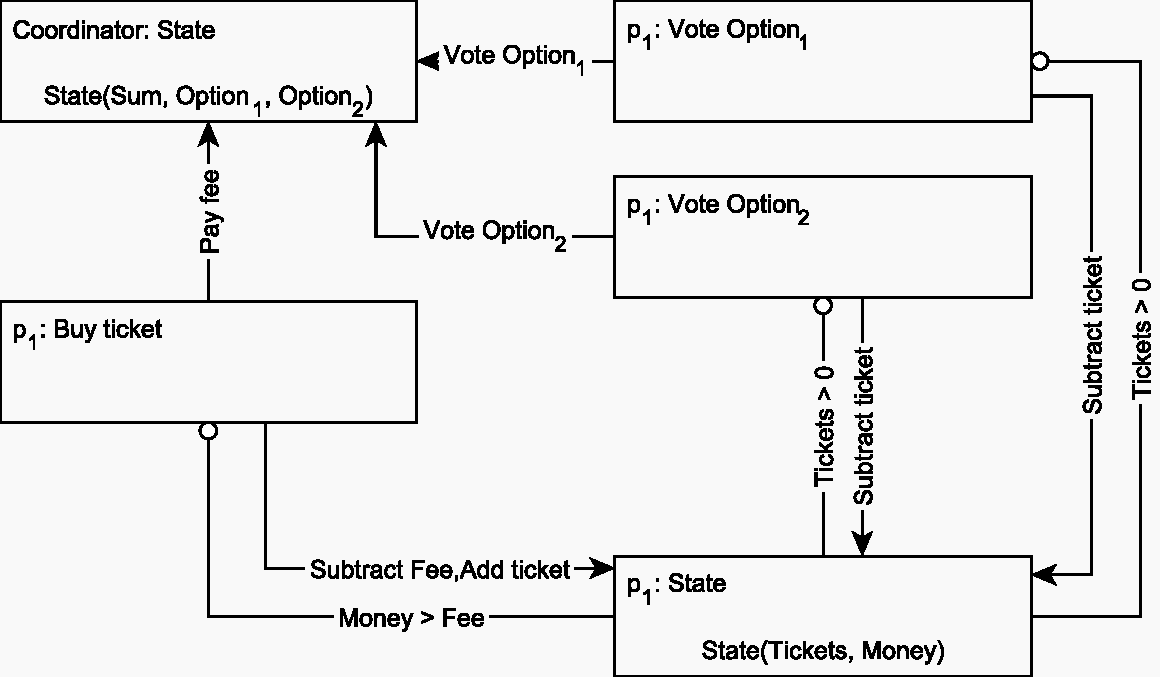
\includegraphics[scale=0.5]{figures/dao-simple.pdf}
\end{frame}

\begin{frame}{Smart contracts}{Parametrised DAO}
	\centering
	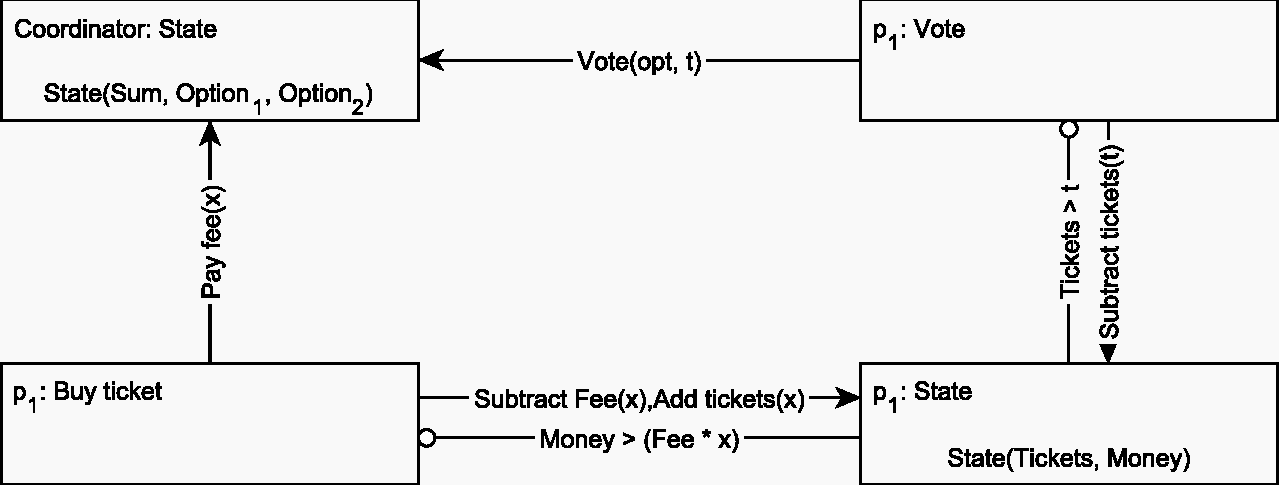
\includegraphics[scale=0.5]{figures/dao-parametrised.pdf}
\end{frame}

\begin{frame}{Summary}%mikkel
	\begin{itemize}
		\item Relies on Intel hardware, code and secrecy
		\item Requires TPM on all clients
	\end{itemize}
\end{frame}

\end{document}
